\documentclass[12pt]{extarticle}
\usepackage[utf8]{inputenc}
\usepackage{cite}
\usepackage{amsmath}
\usepackage{hyperref}
\usepackage{graphicx}
\graphicspath{{./report/image/}}
\usepackage{etoolbox}
\apptocmd{\sloppy}{\hbadness 10000\relax}{}{} 
%^This is here to fix long URLs in refs.bib throwing underfull hbox errors

\title{A Parallel Application of the Fourier Transformation}
\author{Justin Spidell -- Brett Sumser}
\date{December 2021}

\begin{document}

\maketitle
\newpage

\begin{abstract}
\normalsize %Makes the abstract normal size
	In this project we implemented many versions of the Fourier Transform. 
	Namely, we implemented a parallel Discrete Fourier Transform (hereby referred to as the DFT), a iterative version of the Fast Fourier Transfrom (hereby referred to as the FFT), and a MPI version of the Parallel DFT. 
	Our main results in this project concerned converting analog signals into digital (discrete) signals, then preforming a Fourier Transform on the signals to ascertain the pitches in the original audio.
	% insert something about image proccessing. 
    Our project was written in C++ and a little bit of python, and we used the openmp and the openmpi libraries.
\end{abstract}

\newpage
\section*{Introduction}

	The Fourier Transform is an important mathematical concept.	
	Discovered in 1822 by Joseph Fourier, it has applications in digital signal processing, convolution in neural networks, image recognition and even speech processing.
    A Fourier Transform can be described as a "mathematical operation that changes the domain (x-axis) of a signal from time to frequency," \cite{Maklin:2019}. 
    The Fourier transform is denoted by adding a circumflex to the symbol of a function:

	\begin{align*}
		f \rightarrow \hat{f}
	\end{align*}

	The Fourier transform is defined as:

	\begin{align}
		\hat{f} (\xi)= \int^{\infty}_{-\infty}f(x) e^{-2 \pi i x \xi}dx
	\end{align}
	
	Where x represents time, and $\xi$ represents frequency.
	\\

    For our purposes, specifically the conversion of signals and image processing, we need to use the non-continuous (discrete) version of the Fourier Transform.
    Unfortunately, the DFT is on the slower side for algorithms, being performed in $O(n^2)$.
    It is defined as:
    
	\begin{align*}
		Let\ x_{0},\ ..., x_{N-1}\ be\ complex\ numbers,
	\end{align*}
	\begin{align}
		X_{k} = \sum_{n=0}^{N-1}x_{n}e^{\dfrac{-2 i \pi k n}{N}}\ \ \ k = 0,\ ...,\ N-1
    \end{align}
   
	Using Euler's identity, we can transpose the function to:
	
	\begin{align*}
		Let\ x_{0},\ ..., x_{N-1}\ be\ complex\ numbers,
	\end{align*}
	\begin{align}
		X_{k} = \sum_{n=0}^{N-1}x_{n} \cos{(\dfrac{-2 \pi k n}{N})} + i\sin{(\dfrac{-2 \pi k n}{N})}\ \ \ k = 0,\ ...,\ N-1
    \end{align}
    
    This will be our main implementation, as it neatly separates the real and imaginary components.
   \\
   
   	To achieve a FFT, we must go a step further.
   	By splitting the DFT into two subsections, we can achieve a DFT with less computations and better speeds.
	The FFT is much faster than the DFT, being performed in $O(n\log{}n)$ time.
	The FFT can be easily implemented using a recursive or iterative programming method, but there are benefits to using an iterative approach; Mainly the ability to be parallelized.
    The FFT is a radix-2 algorithm, meaning that it is really two interleaved DFTs of size $N/2$.
    The FFT can be defined as:
    
    \begin{align*}
		Let\ x_{0},\ ..., x_{N-1}\ be\ complex\ numbers,
	\end{align*}
	\begin{align*}
		X_{k} = \sum_{m=0}^{N / 2 - 1}x_{2m}e^{\dfrac{-2 i \pi k m}{N / 2}} - e^{\dfrac{-2 i \pi k}{N}} + \sum_{m=0}^{N / 2 - 1}x_{2m + 1}e^{\dfrac{-2 i \pi k m}{N / 2}}
	\end{align*}
	\begin{align*}
		X_{k + N / 2} = \sum_{m=0}^{N / 2 - 1}x_{2m}e^{\dfrac{-2 i \pi k m}{N / 2}} - e^{\dfrac{-2 i \pi k}{N}} + \sum_{m=0}^{N / 2 - 1}x_{2m + 1}e^{\dfrac{-2 i \pi k m}{N / 2}}
	\end{align*}
	\begin{align}
		 for \ k = 0,\ ...,\ N-1
    \end{align}
    
    %lol
    Of course our implementation applies Euler's Identity to split the function into real and imaginary components, but this will be left as an exercise to the reader.

\section*{Methodology}

	\subsection*{Implementation of the Algorithms}
		As stated previously, we used C++ to implement our various Fourier Transforms.
		Our most basic DFT algorithm was written with two loops, calculating a sum using every input for each value in our output.
		\\

		The FFT (Cooley-Tukey) takes a much different form.
		In this algorithm, we first must pad the input with 0's, this will produce some unavoidable error into the calculation, however it is negligible.
		We have to pad with 0's because of the nature of the FFT, it is a radix-2 algorithm, and must have an input that is a power of two.
		This is expensive on our time, but the benefit we get from using the FFT outweighs the cost.
		Next, we must bit reverse the indicies of the input.
		This means given an input of size 16 (4 bits) that a number located at index 3 $(0011)$ must be switched with the number located at 12 $(1100)$.
		Although bit operations are very fast, this still can be an expensive operation. 
		However, the speed of the FFT far outweighs the cost of the re-indexing.
		Finally, We start the main body of the FFT.
		We used an iterative implementation, so the main body consists of two for loops, one controlling the flow of the algorithm, and the other calculating the partial sums.
		
		

\subsection*{Parallization} 
    
    There are a few different directions to explore when developing a more
    parallized implementation of the Fourier Transform. 
    According to Anthony Blake in his thesis paper titled "Computing the Fast Fourier Transform on SIMD Microprocessors",
    use of the FFT algorithm is extremely widespread in multiple disciplines. He goes on to state that 
    "use of the FFT is even more pervasive, and it is counted among the 10 algorithms that have had the greatest influence 
    on the development and practice of science and engineering in the 20th century," \cite{Blake:2012}.
    The widespread use of the FFT algorithm provides great evidence for the need to optimize for different applications,
    and to understand the methods that can be used to achieve this.
    Two methods of Parallelization that stand out in particular are SIMD, and multithreading.
   
    After some preliminary research into a multithreading implementation of FFT\cite{Thulasiraman:2021}, it seems there are
    possible multithreaded implementations of the FFT. Based on the previously cited source, Thulasiraman et al. picked two 
    different algorithmic approaches to investigate. The first is what they referred to as a sender-initiated algorithm based
    on the Cooley-Tukey FFT algorithm. The Cooley-Tukey algorithm is the most common of the FFT variations, recursively breaking
    the DFT into $N_1$ DFTs of size $N_2$, multiplying by complex roots of unity, and performing $N_2$ DFTs of size $N_1$.
    
    The second is stated as a sender-initited algorithm, utilizing a thread pool fixed at compile time. 
    The amount of threads is equal to $N/B$, with $B$ being the block list for a list of contiguous data pieces. 
    Threads are then distributed between processors round-robin style, which enables load balancing across available processors.
    In the end, each processor will perform an FFT computation on $B$ data pieces.
    This version of the algorithm seems like it may be applicable for use on the University of Oregon supercomputer.

\subsection*{SIMD}
    
    Single Instruction Multiple Data prcoessors are also known as vector processors, and allow a single instruction
    to process multiple pieces of data in the same clock cycle. The way that SIMD works is by packing several pieces of data
    into one data word. This allows the instruction loaded to act on each piece of data from a single instruction.
    This has applications in situations where large amounts of data are being manipulated. With respect to the Fourier Transform,
    this can be applied to image manipulation, audio processing, or other functions.

    According to this post\cite{Konstantin:2020} on StackOverflow, C/C++ contains SIMD functions called vector intrinsics.
    These are implemented in the compiler, allowing them to load orders of magnitude faster than common library functions. 
    The found that they could use these intrinsics to produce code up to four times faster, and even more in certain cases!
    For this project, getting a handle on these intrinsics would allow for an increased knowledge in C/C++, while also providing
    experience in possible future scenarios with performance critical code.

\subsection*{Application}
	We plan to use our FFT implementation to compress images and audios. 
	We will test our implementations speed, comparing with industry standards, and loss, by comparing with the originals. 
	This process will all be automated, taking place on the University of Oregon's supercomputer. 
	We hope to achieve something similar in time complexity and error to commonly found compression software, however this may be a hard goal to reach. 
	
	We will also test our FFT implementation by converting analog audio to digital, and comparing for loss. 
	This is a less intensive but still productive test, being our original goal and very applicable to a real life scenario. 
	
	Overall this FFT implementation will have many functions and possible applications, but only testing a few we hope to create an algorithm that is effective and efficient.
\subsection*{Difficulties}
	Everything did not go as smoothly as planned for the project. There were problems encountered with parallelizing aspects of the 
	project, including various issues with image loading, MPI, and attempting to implement SIMD for increased performance.

	\subsubsection*{Image Loading}
	With regards to loading image data for transforming, there were a couple of difficulties. The Fourier Transform can only transform images
	that are in greyscale, so it makes sense to also look for ways to apply parallelism to the conversion of images to grayscale.
	The first issue encountered was finding a library that was 
	simple to use with little overhead and dependencies to get running. The first attempted library to use was \href{https://opencv.org/}{OpenCV}.
	
	\subsubsection*{SIMD/Intrinsics}
	After discussing the merits of SIMD and Instricsics in C++ with Professor Choi, we reached the decision to focus developement time into
	MPI. With the nature of converting grayscale images for use in the Fourier Transform, the RGB pixels need to be summed, and then the average
	of that value is applied to each RGB component. SIMD could be used to sum the first 2 RGB components, provided that they are memory aligned. 
	However, you would still need to add the last RGB compenent, and then perform a division and assign the value to all of the pixel values.
	It was brought to our attention that although this is possible, the speedup overall would probably not really be worth the effort to get it
	running.

	\subsubsection*{MPI}

\section*{Results}

Utilizing our implementation of the Discrete Fourier Transform, we were able to successfully filter out individual pitches in musical
chords. 

\begin{center}
\begin{figure}
  \includegraphics[scale=0.75]{pitchgraph.png}
  \caption{Graph of Results}
\end{figure}
\end{center}

With a N = 2^17 or 131072, testing on Talapas, we got these times:
\subsection*{Speed}
%With a N = 2^17 or 131072, testing on Talapas, we got these times:
DFT: 				N/A
PDFT: 				60.4222 seconds
Cooley-Turkey: 		0.14108 seconds
// (critical) Cooley-Turkey: 	2.32468 seconds
// (locks) Cooley-Turkey: 	1.31673 seconds
Industry Standard (numpy):	0.00323 seconds

\subsection*{Audio}
Utilizing our implementation of the Discrete Fourier Transform, we were able to successfully filter out individual pitches in musical
chords.

\begin{figure}[h]
  \includegraphics[scale=0.75]{./images/pitchgraph.png}
  \caption{Graph of Results}
\end{figure}

\section*{Conclusion}
	By creating a implementation of the Fast Fourier Transform, we hope to gain insight into modern image and audio compression software, as well commonly found analog to digital conversion software.
    We will attempt to implement a more sophisticated parallelized version of the FFT, using concepts applied from class such as SIMD and multithreading/processing.
    We are excited to be able to have access the hardware capable of applying these concepts for parallelized computing.
	The University of Oregon's supercomputer will be applied for testing and use of our implementation, hopefully with success. 
	This is a lofty goal, and will take a good amount of work, but the end result will be something to be proud of.

\bibliographystyle{plain}
\bibliography{refs} % Entries are in the &quot;refs.bib&quot; file</code></pre>

\end{document}